\documentclass{article}
\usepackage[utf8]{inputenc}
\usepackage[]{graphicx}
\usepackage{float}

\begin{document}
\section*{Practical 1}%
\subsection*{Exercise 2}%
\label{sub:tp1ex2}
The size of the graph is calculated by iterating over the text file and
counting the number of lines containing pairs of integers.
Note that this is to be used on raw graphs, as cleaned ones already contain the
number of nodes and edges on the first line.
As a result of this and the fact that we avoid storing the edges in memory, the
program doesn't account for potential duplicates.

\subsection*{Exercise 3}%
\label{sub:tp1ex3}
The program first counts the number of lines using ``wc -l", to tell how much
memory it should allocate for the edge list, then we iterate over each line
and add the edges to the list in the correct order.
(tail is strictly smaller than head)\\
We then sort the edge list in lexicographical order.
(the order is based on tail of edge, and in case of equality, on the head of the
edge)\\
We iterate over the edge list to count the number of non duplicate edges,
and write the number of nodes and number of edges to a new text file.\\
We iterate once again on the list of edges and save them to a new text file,
skipping over duplicates. Note that node indices are shifted so that they start
from 0.

\subsection*{Exercise 4}%
\label{sub:tp1ex4}
We read the number of nodes and the number of edges from the cleaned files, and
allocate memory for a list of node degrees.\\
We iterate over the (cleaned) file of list of edges, and for each edge, we
increment the degrees of its tail and its head.

\subsection*{Exercise 5}%
\label{sub:tp1ex5}
We read the number of nodes and the number of edges from the cleaned files, and
allocate memory for a list of edges and a list of node degrees.\\
We first calculate the degrees of nodes.\\
Then we iterate over the edge list and calculate the desired quantity.
\begin{table}[!ht]
    \centering
    \label{tab:label}
    \begin{tabular}{lrrr}
        Graph & $Q_G$ & degree computation& $Q_G$ computation\\
        Email&
        103747042&
        0.001894s&
        0.000026s\\
        Amazon&
        103415531&
        0.136159s&
        0.003211s\\
        Live Journal&
        789000450609&
        5.016865s&
        0.126856s\\
        Orkut&
        22292678512329&
        17.231983s&
        0.430236s\\
        Friendster&
        379856554324947&
        389.599227s&
        24.310711s\\
    \end{tabular}
\end{table}

\subsection*{Exercise 6}%
\label{sub:tp1ex6}
We compute the degree list and save it to a file, we then count the number of
occurences of each value and plot the distribution.

\begin{figure}[H]
    \centering
    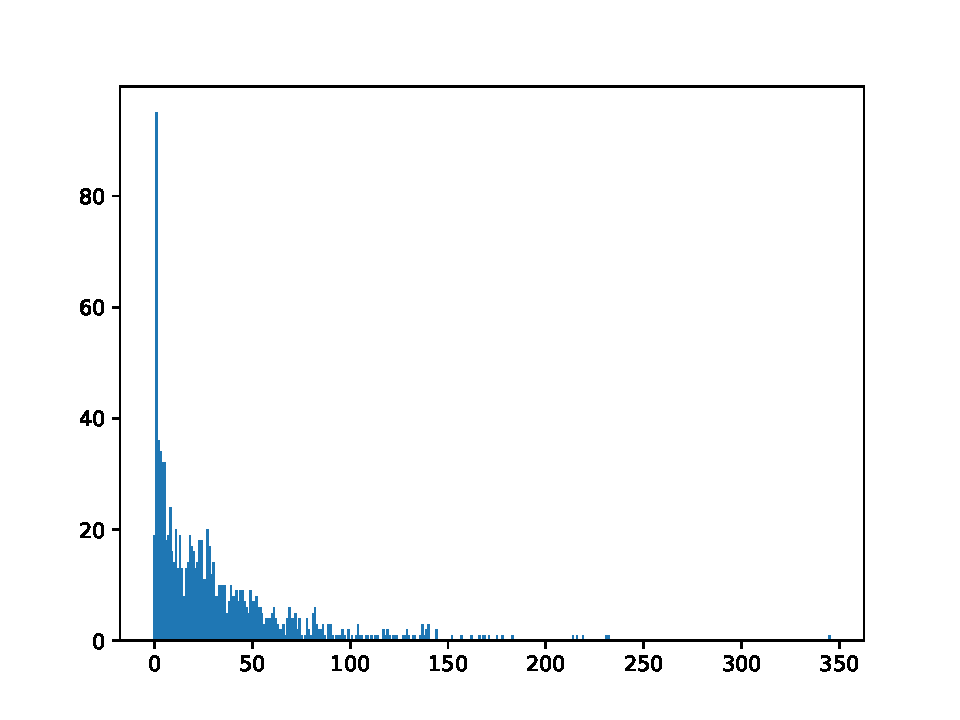
\includegraphics[width=0.8\textwidth]{plots/email-Eu-core.pdf}
    \caption{Email graph degree distribution}
    \label{fig:email-deg}
\end{figure}

\begin{figure}[H]
    \centering
    \includegraphics[width=0.8\textwidth]{plots/{com-amazon.ungraph}.pdf}
    \caption{Amazon graph degree distribution}
    \label{fig:amazon-deg}
\end{figure}

\begin{figure}[H]
    \centering
    \includegraphics[width=0.8\textwidth]{plots/{com-lj.ungraph}.pdf}
    \caption{Live Journal graph degree distribution}
    \label{fig:lj-deg}
\end{figure}

\begin{figure}[H]
    \centering
    \includegraphics[width=0.8\textwidth]{plots/{com-orkut.ungraph}.pdf}
    \caption{Orkut graph degree distribution}
    \label{fig:orkut-deg}
\end{figure}

\begin{figure}[H]
    \centering
    \includegraphics[width=0.8\textwidth]{plots/{com-friendster.ungraph}.pdf}
    \caption{Friendster graph degree distribution}
    \label{fig:friend-deg}
\end{figure}

\subsection*{Exercise 7}%
\label{sub:tp1ex7}
The list of edges is stored ``as is".\\
The adjacency matrix is represented as an array of arrays of char values.
Each array contains a row of the matrix, and each char value contains 8
consecutive elements of the row.\\
Degrees of nodes are first calculated, then the adjacency array is stored as
specified in the course.

\subsection*{Exercise 8}%
\label{sub:tp1ex8}
We allocate an array to contain the component index of each node, initialized
to -1, and we set the count of components to 0.\\
We iterate over the nodes, and whenever a component of -1 is found, we set its
compoenent index as well as the ones of all the nodes connected to it (found by
a breadth-first search) to the current count.
We then increment the compoenent count by 1.

\begin{table}[htpb]
    \centering
    \begin{tabular}{lrr}
        Graph & \% nodes in largest component & Diameter lower bound\\
        Email&
        98.109453\%&
        7\\
        Amazon&
        61.045008\%&
        47\\
        Live Journal&
        99.044330\%&
        21\\
        Orkut&
        99.993979\%&
        10\\
        Friendster&
        52.555613\%&
        37\\
    \end{tabular}
\end{table}

\section*{Practical 2}%
\label{sec:tp2}
\subsection*{Exercise 1}%
\label{sub:tp2ex1}
We read the directed edge list and store it as an adjacency array.
The matrix vector product and the PageRank algorithm are implemented as
specified in the course.\\
For $\alpha = 0.15$, the algorithm converges in 16 iterations.\\
Top 5 pages
\begin{itemize}
    \item United States
    \item United Kingdom
    \item Germany
    \item 2007
    \item 2006
\end{itemize}
Bottom 5 pages
\begin{itemize}
    \item WCXL
    \item WGCC-FM
    \item WAFJ
    \item WBFR
    \item Leroy Township, Michigan
\end{itemize}

\subsection*{Exercise 2}%
\label{sub:tp2ex2}
We use linear scales for degrees and log scales for pagerank values, since they
take values close to 0 with different orders of magnitude.

\begin{figure}[H]
    \centering
    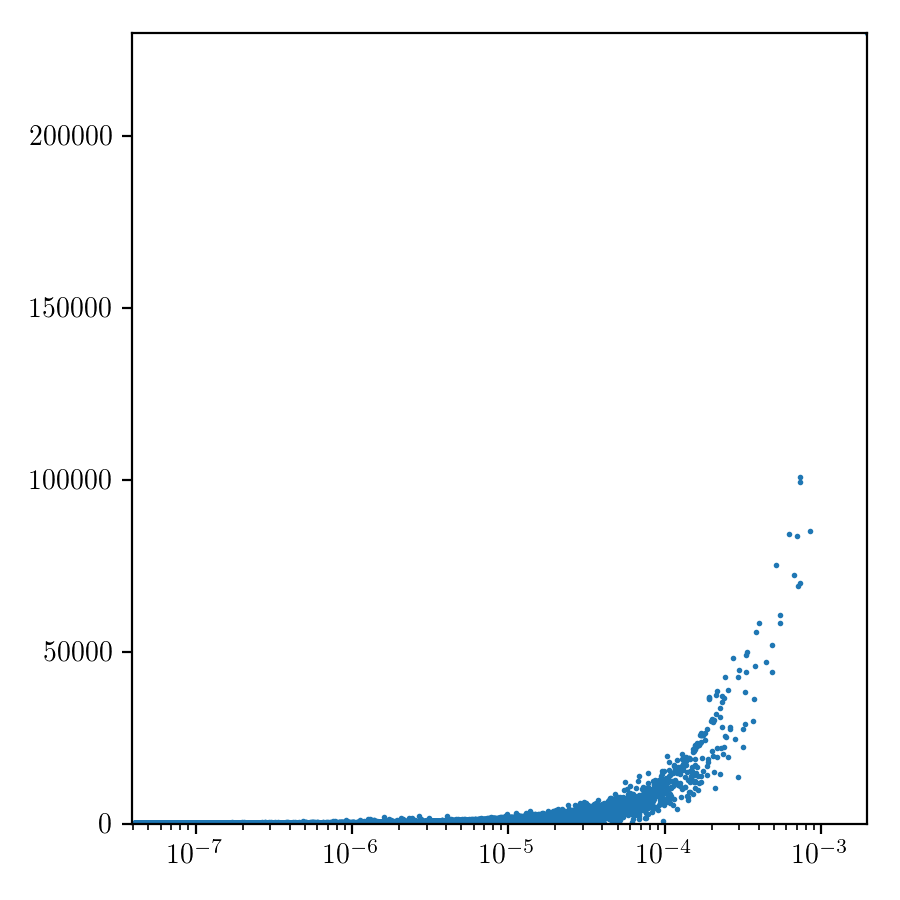
\includegraphics[width=0.65\textwidth]{plots/1.png}
    \caption{$x =$ PageRank with $\alpha = 0.15$, $y = $ in-degree}
    \label{fig:1}
\end{figure}

\begin{figure}[H]
    \centering
    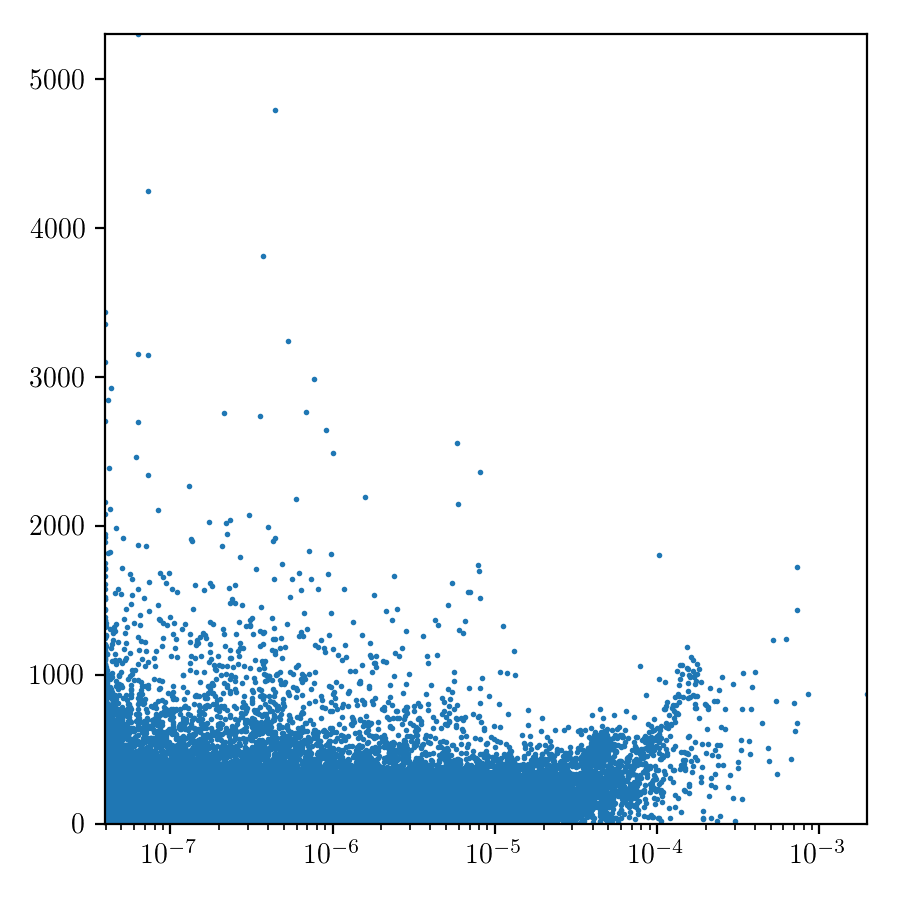
\includegraphics[width=0.65\textwidth]{plots/2.png}
    \caption{$x =$ PageRank with $\alpha = 0.15$, $y = $ out-degree}
    \label{fig:2}
\end{figure}

\begin{figure}[H]
    \centering
    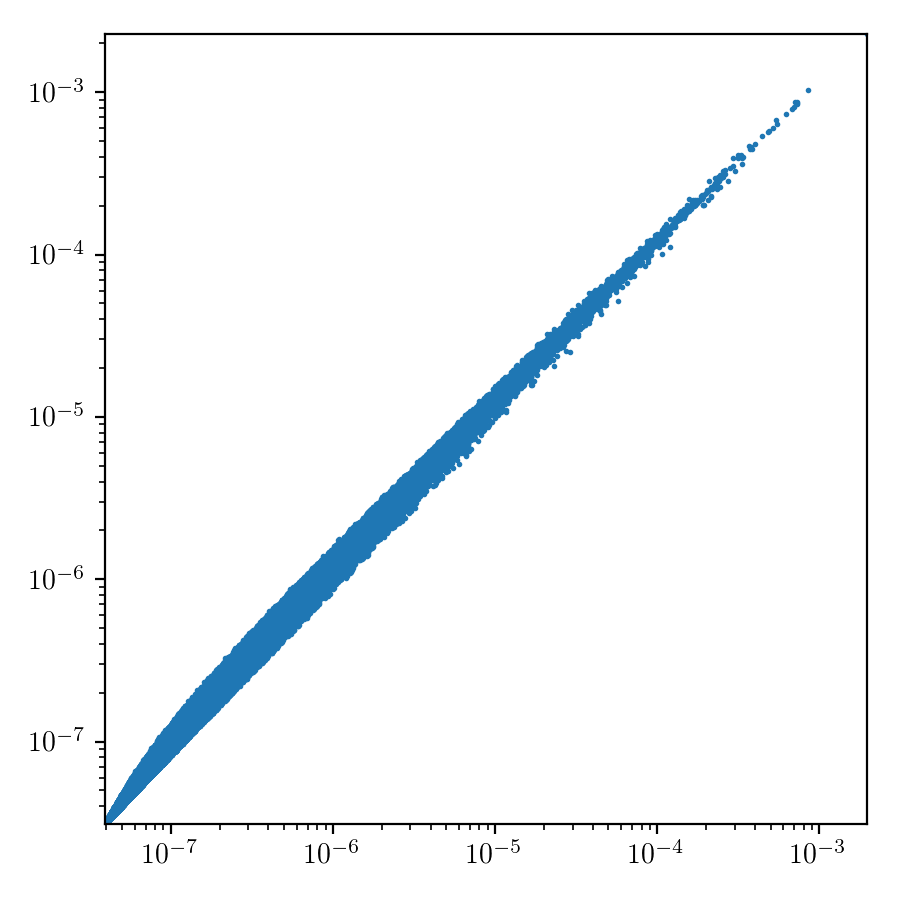
\includegraphics[width=0.65\textwidth]{plots/3.png}
    \caption{$x =$ PageRank with $\alpha = 0.15$, $y = $ PageRank with $\alpha = 0.1$}
    \label{fig:3}
\end{figure}

\begin{figure}[H]
    \centering
    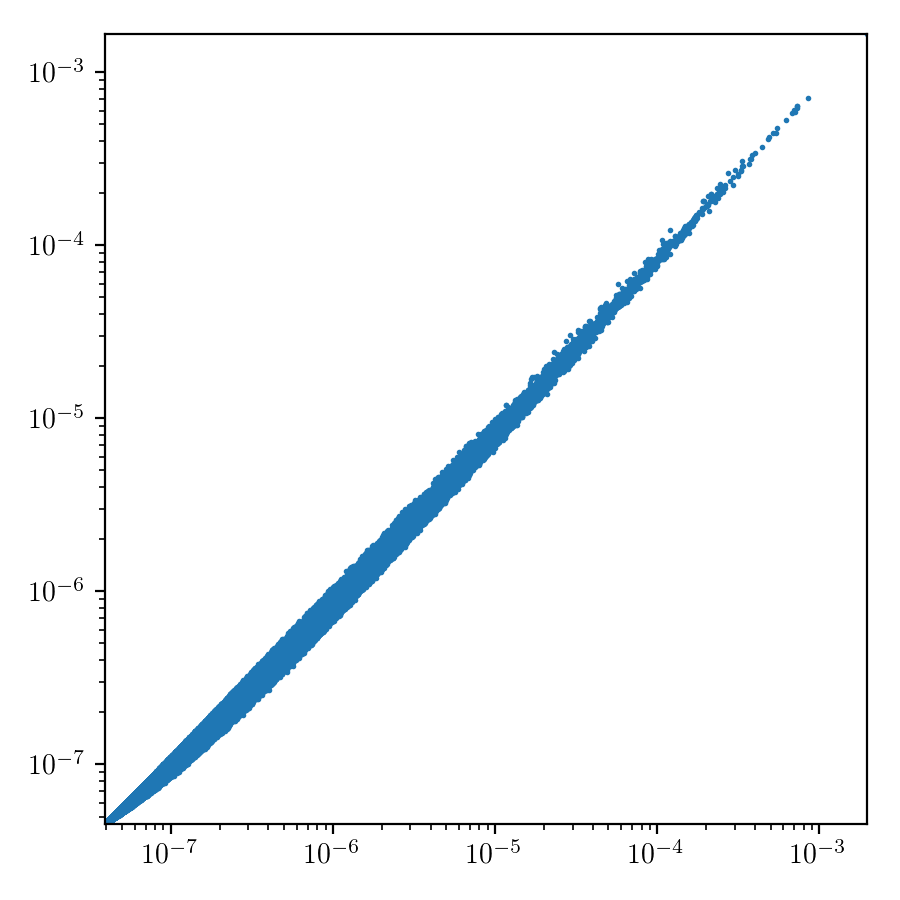
\includegraphics[width=0.65\textwidth]{plots/4.png}
    \caption{$x =$ PageRank with $\alpha = 0.15$, $y = $ PageRank with $\alpha = 0.2$}
    \label{fig:4}
\end{figure}

\begin{figure}[H]
    \centering
    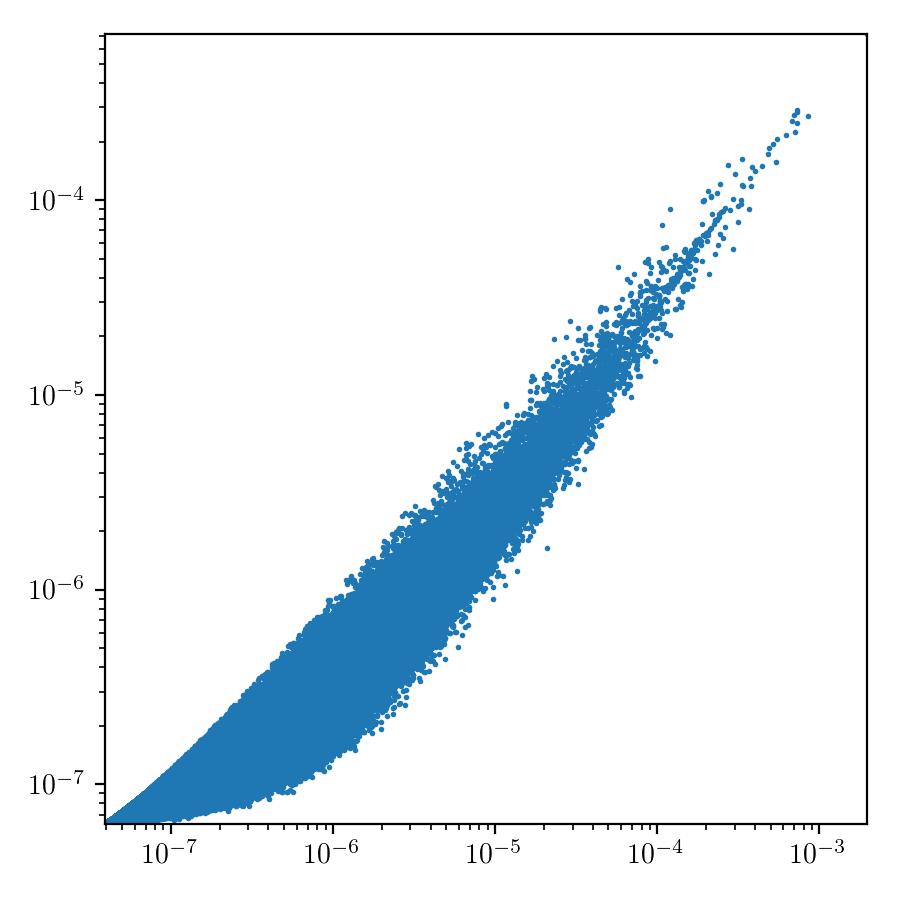
\includegraphics[width=0.65\textwidth]{plots/5.png}
    \caption{$x =$ PageRank with $\alpha = 0.15$, $y = $ PageRank with $\alpha = 0.5$}
    \label{fig:5}
\end{figure}

\begin{figure}[H]
    \centering
    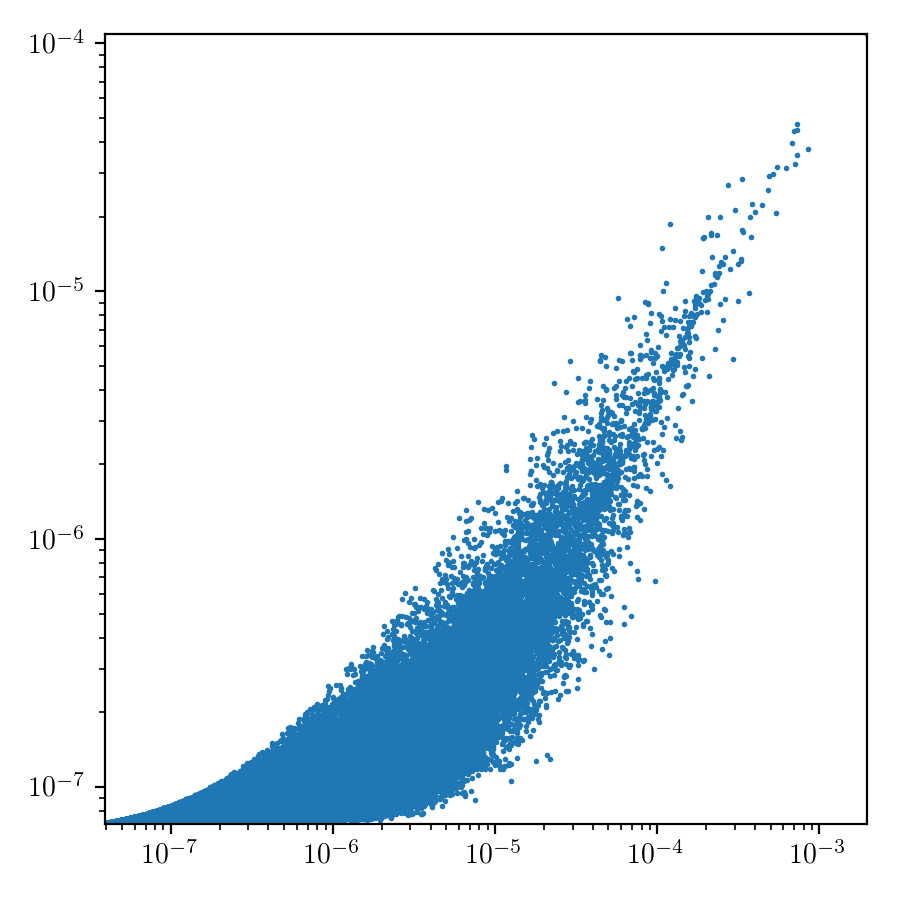
\includegraphics[width=0.65\textwidth]{plots/6.png}
    \caption{$x =$ PageRank with $\alpha = 0.15$, $y = $ PageRank with $\alpha = 0.9$}
    \label{fig:6}
\end{figure}

\subsection*{Exercise 3}%
\label{sub:tp2ex3}
\begin{table}[!ht]
    \centering
    \begin{tabular}{lrr}
        Graph & Running time & Core value\\
        Email&
        0.000548s&
        34\\
        Amazon&
        0.167125s&
        6\\
        Live Journal&
        4.625723s&
        360\\
        Orkut&
        16.438648s&
        253
    \end{tabular}
\end{table}

\section*{Practical 3}%
\label{sec:tp3}
\subsection*{Exercise 1}%
\label{sub:tp3ex1}
Increasing $ \frac{p}{q} $ makes the community structure more evident.
And in the limit case of $ \frac{p}{q} \to 1 $, the communities become
indistinguishable.

\subsection*{Exercise 2}%
\label{sub:tp3ex2}
The label propagation algorithm is implemented as specified in the course.

\subsection*{Exercise 3}%
\label{sub:tp3ex3}
The communities are determined as follows:\\
For each node, we find the neighbor with minimal degree and require that they
be in the same community.
This is repeated until the graph reaches a stable state and communities stop
changing.

The intuition behind is that the nodes who have connections outside their
community tend to have a greater degree than those with connections limited
to their own community.
This tends to work well on graphs with clear community structure.

\end{document}
